\section{NSW Readout Electronics and Detector Instrumentation}
\label{sec:nsw_elx}

To a very large extent, high-performance detectors are realised and made
possible only by their interfacing to equally high-performance readout electronics;
that is, high quality electronics enable high quality detectors.
{\color{red}{See Appendix XXX for a discussion on the general characteristics of
detector readout electronics.}}
In this section, therefore, an introduction to the frontend electronics\footnote{`Frontend' electronics
are those housed directly on the detectors themselves and are responsible for reading out the
detector signals and potentially many other responsibilities, such as calibration, configuration, and
detector controls (temperature monitoring, etc...). `Backend' electronics refer to those
not necessarily located in the experimental cavern housing the detectors but are in the nearby
service areas or on the surface (c.f. Figu:e~\ref{fig:p1}) and are dedicated, for example, to the implementation of detector trigger logic
and data decoding and event building (i.e. gathering all data from detector hits associated with a given event).}
relevant to the NSW will be given.
There is a large set of both frontend and backend electronics specifically
designed and constructed for the NSW~\cite{NSWFrontEndChristos}.
Here, though, we will focus primarily on the frontend electronics.
The NSW frontend electronics revolve around the operation of a family
of rather complex application specific integrated circuits (ASICs),
each targetting a specific (set of) purpose(s) related to data-acquisition or
constructing trigger primitives:
%including a family of application specific integrated circuits (ASICs):

\begin{description}
    \item[] \textbf{VMM}~\cite{VMM1GDG,VMMASIC,VMM3George} Frontend readout ASIC used for precision and fast trigger data signal collection in both MM and sTGC detectors
    \item[] \textbf{ROC}~\cite{NSWTDR,NSWFrontEndChristos} `ReadOut Controller' ASIC, responsible for buffering and aggregating precision data from the VMM
    \item[] \textbf{TDS}~\cite{TDS} `Trigger Data Serialiser' ASIC, processes trigger signals from VMMs on the sTGC detectors and prepares trigger primitives for the NSW Level-1 muon trigger logic
    \item[] \textbf{ART}~\cite{NSWTDR,ARTASIC} 'Address in Real Time' ASIC, processes trigger signals from VMMs on the MM detectors and prepares trigger primitives for the NSW Level-1 muon trigger logic
\end{description}

The VMM ASIC is the primary ASIC of the NSW: all other ASICs listed above take as input
the outputs of the VMM and, in this respect, are secondary.
The work of the current author on the NSW frontend electronics is based almost exclusively
on the characterisation and validation of the VMM ASIC.
For these reasons, focus will be given on describing the VMM in Section~\ref{sec:vmm}.
For the interested reader, further information on the ROC, TDS, and ART ASICs is
provided in the references above.
The interface of the NSW frontend electronics to the associated detectors is dictated for the most part
by the geometry, type, and number of the detectors' readout elements (MM: strips, sTGC: strips, wires, and pads)
and foreseen space limitations in the ATLAS detector.
The work in the present thesis concerns the frontend boards related to the MM detectors.
This is mainly due to the fact that the VMM was initially conceptualised as a frontend ASIC specialised
for MPGD detectors and its initial prototypes were studied under this context by the RD51 collaboration
at CERN which is devoted to the development of MPGD technologies, such as the MM detectors.\footnote{For more information
on the RD51 collaboration, visit their homepage: \url{http://rd51-public.web.cern.ch/rd51-public/}.}
In Section~\ref{sec:nsw_boards}, then, a description of the relevant front-end boards used in the
study, validation, and integration of the VMM ASIC, as well as those that will be used in
the MM detectors of the NSW, will be given.
The analgogous VMM-based frontend boards for the sTGC detectors are objectively more complicated than those
of the MM detectors for purely technical and uninteresting reasons.
Their description can be found elsewhere~\cite{NSWTDR}.
{\color{red}{Maybe change how I describe why I am focused on MM detectors etc...}}

\subsection{The VMM ASIC}
\label{sec:vmm}

The VMM is a custom ASIC that can be used in a variety of charge-interpolated tracking
detectors.
There have been several iterations of the VMM over the years, starting with the VMM1~\cite{VMM1GDG} and
moving up to the VMM3~\cite{VMMASIC,VMM3George}.
An illustration of the evolution of complexity of the VMM ASIC is shown in Figure~\ref{fig:vmms_silicon}.
The VMM1 was a purely analog readout ASIC considered to be a prototype of the initial VMM functionalities.
The VMM2 was an extensive upgrade of the VMM1, adding the necessary digital logic and functional blocks
required for the NSW detectors.
The VMM3 is the final version of the ASIC\footnote{In actuality, there have been two versions of the
VMM3: the VMM3 and the `VMM3a'. The VMM3a is the true final version that will be used in the NSW
and addresses issues found during the testing and validation of the first round of the VMM3 production}
providing enhanced functionality required for data taking in ATLAS
as well as addressing bugs found in the operation of the VMM2
VMM3 is the version that will be used
in the NSW once installed in ATLAS.
The VMM implements all logic using triple modular redundancy (TMR) to protect itself
from single event upsets (SEUs) that are expected to be quite common in the
harsh radiation environments in which the NSW will be situated.

The VMM is composed of 64 discrete frontend channels, each to be connected to a detector
readout element.
A block diagram illustrating the functional blocks of the VMM3 and its channels is
shown in Figure~\ref{fig:vmm3_channel}.
Each channel has a dedicated charge amplifier (`CA' in Figure~\ref{fig:vmm3_channel}) and signal
shaping functionality,
threshold discriminator, test-pulse injection capacitor with adjustable amplitude provided
by a 10-bit digital-to-analog converter (DAC), and precise signal amplitude and timing measurements digitally readout via
internal per-channel analog-to-digital converters (ADCs).
The amplitude measurement of the input pulse is digitised by a 10-bit ADC (`PDO', for `peak detector output', in Figure~\ref{fig:vmm3_channel})
and the timing estimation of the signal pulse's peak is digitised by an 8-bit ADC (`TDO', for `time detector output', in Figure~\ref{fig:vmm3_channel}).
The digitised output of these amplitude and timing measurements are calculated by these
internal ADCs within 200\,ns and stored in internal buffers of the VMM.
The buffered data is stored until selected for readout by another ASIC housed on the same frontend
board as the VMM, the ROC, based on the buffered data's bunch crossing.

In addition to the precision data useful for reconstructing high-level muon tracks provided by
the PDO and TDO measurements, the VMM can also operate at a faster mode used for
providing data needed for the building of trigger primitives.
In the trigger mode referred to as the `Address-in-Real-Time' (ART) mode,
the VMM outputs the \textit{first} channel address (i.e. MM strip number) on which
an above-threshold peak was detected.
An alternative trigger mode relies on the VMM's ability to perform a fast digitisation of
the signal pulse amplitude using a 6-bit ADC, providing a coarse but rapid measurement
of the signal amplitude.
Additionally, the VMM can output fast timing signals, such as a flag indicating a signal over threshold (`Time-Over-Threshold', or TOT as in Figure~\ref{fig:vmm3_channel}).
The ART trigger scheme is used for the MM trigger primitives and the combination
of the coarse 6-bit amplitude and fast-timing signals is used for building the
sTGC trigger primitives.

One of the powers of the VMM is its highly configurable nature.
This, of course, makes the ASIC quite complex in terms of its design but is
advantageous in terms of its range usefulness.
Some of the main configurable items are the peaking (integration) time of the signal shaper
(25, 50, 100, and 200\,ns), adjustable thresholds per-VMM configured by an on-VMM
10-bit (DAC),
adjustable channel gains (0.5, 1, 3, 4.5, 6, 9, 12, and 16\,mV/fC),
time-to-amplitude conversion (TAC) ramp time (60, 100, 350, and 650\,ns) relevant for the timing measurements,
and channel threshold trimmers provided by 5-bit DACs that adjust each channel's individual
threshold around the globally (per-VMM) configured threshold.
The VMM input can also be configured to handle either positive or negative input
signals.
This latter fact is necessary for the NSW, in which the sTGC and MM detectors
will induce signals of opposite polarity on their readout elements.\footnote{The MM strips and
sTGC wires produce signals of opposite polarity as the sTGC strips and pads.}

\begin{figure}[!htb]
    \begin{center}
        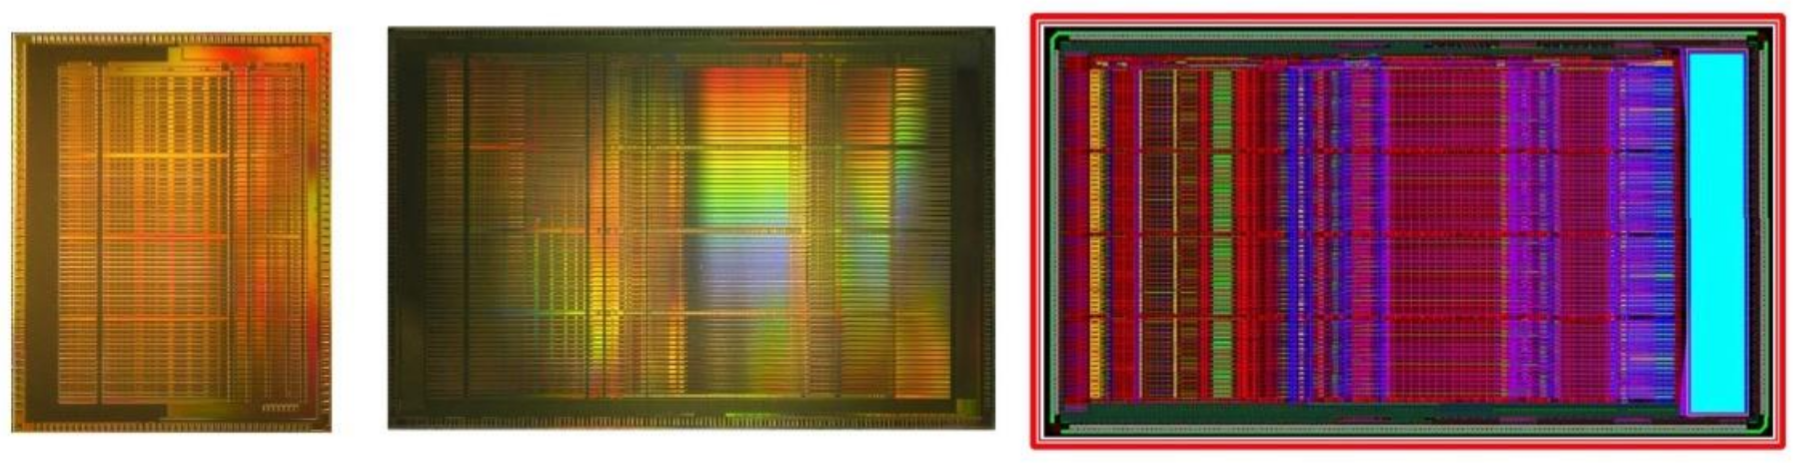
\includegraphics[width=0.8\textwidth]{figures/nsw/vmm/vmms_silicon}
        \caption{
            Evolution of the VMM ASIC.
            Shown are the silicon dies or routing of the the VMM1 (\textbf{\textit{left}}), to the VMM2 (\textbf{\textit{middle}}), and 
            the VMM3 (\textbf{\textit{right}}), the final version that will be used in the NSW.
            The VMM1 has an area of 50\,mm$^2$ with $\approx 500$\,k MOSFETs, the VMM2 area is 115\,mm$^2$ with $>5$\,M MOSFETs,
            and the VMM3 area is 130\,mm$^2$ with $>6$\,M MOSFETs.\protect\footnotemark%
        }
        \label{fig:vmms_silicon}
    \end{center}
\end{figure}
\footnotetext{`MOSFET' stands for metal-oxide-semiconductor field-effect  transistor', the most widely used transistor in digital and analog electronics.}

\begin{figure}[!htb]
    \begin{center}
        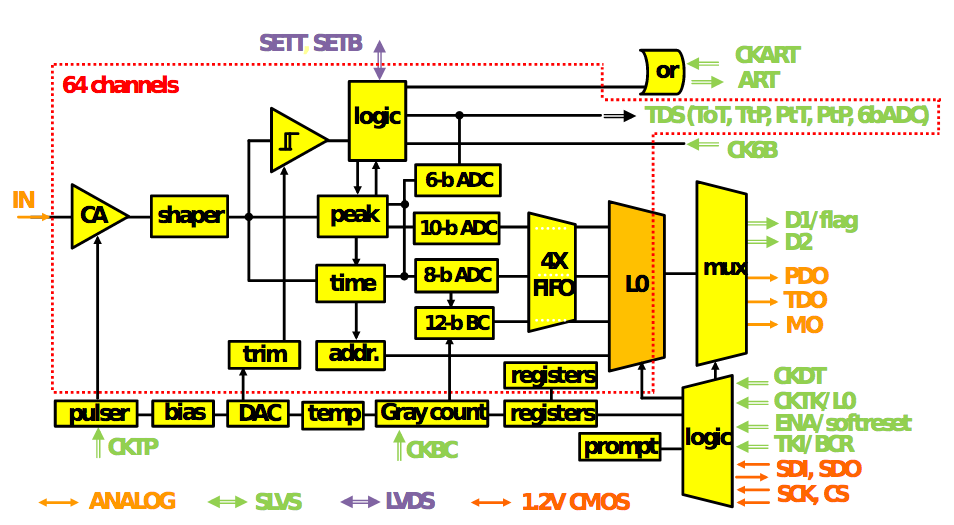
\includegraphics[width=0.8\textwidth]{figures/nsw/vmm/vmm3_channel}
        \caption{
            Architecture of the VMM3.
            The items contained within the dotted red line are repeated
            for each of the 64 channels of the VMM.
        }
        \label{fig:vmm3_channel}
    \end{center}
\end{figure}

\subsection{Front-end Boards for the NSW}
\label{sec:nsw_boards}
